
\begin{figure}
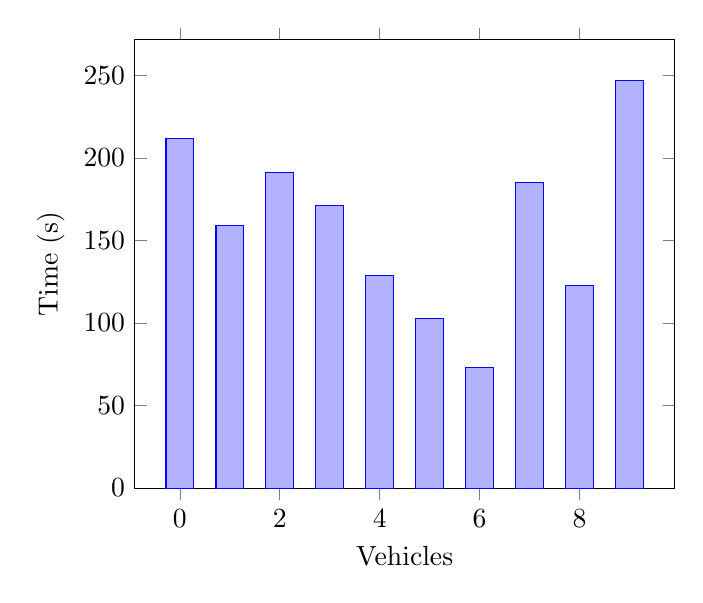
\begin{tikzpicture}
\begin{axis}[
legend style={anchor=west},
xlabel=Vehicles,
ylabel=Time (s),
ymin=0,
ybar,
]
\addplot coordinates {
(0, 212)
(1, 159)
(2, 191)
(3, 171)
(4, 129)
(5, 103)
(6, 73)
(7, 185)
(8, 123)
(9, 247)
};

\end{axis}
\end{tikzpicture}
\label{tik:0:18_N, 18_N.-60, 17_N, 15_S, 15_S.-30, 13_N, 13_N.-40, 11_N, 8_N, 7_N, 7_N.-60, 6_V}
\caption{0 percent diving with GSC on route $18_N, 18_N.-60, 17_N, 15_S, 15_S.-30, 13_N, 13_N.-40, 11_N, 8_N, 7_N, 7_N.-60, 6_V$}
\end{figure}
